% /**
%  * A template for homework files in math classes. The 
%  * packages and newcommands are a good starting point.
%  *
%  * Author: James K. Pringle
%  * E-mail: jameskpringle@gmail.com
%  * Last Changed: 26 May 2013
%  *
%  * "LaTeX countains the increasing union of MS Word"
%  */
%~~~~~~~~~~~~~~~~~~~~~~~~~~~~~~~~~~~~~~~~~~~~~~~~~~~~~~~~~%
%%%%%%%%%%%%%%%%%%%%%%%%%%%%%%%%%%%%%%%%%%%%%%%%%%%%%%%%%%%
%                                                         %
%                        PAGE SETUP                       %
%                                                         %
%%%%%%%%%%%%%%%%%%%%%%%%%%%%%%%%%%%%%%%%%%%%%%%%%%%%%%%%%%%
\documentclass[letterpaper, 12pt]{article}\usepackage[]{graphicx}\usepackage[]{color}
%% maxwidth is the original width if it is less than linewidth
%% otherwise use linewidth (to make sure the graphics do not exceed the margin)
\makeatletter
\def\maxwidth{ %
  \ifdim\Gin@nat@width>\linewidth
    \linewidth
  \else
    \Gin@nat@width
  \fi
}
\makeatother

\definecolor{fgcolor}{rgb}{0.345, 0.345, 0.345}
\newcommand{\hlnum}[1]{\textcolor[rgb]{0.686,0.059,0.569}{#1}}%
\newcommand{\hlstr}[1]{\textcolor[rgb]{0.192,0.494,0.8}{#1}}%
\newcommand{\hlcom}[1]{\textcolor[rgb]{0.678,0.584,0.686}{\textit{#1}}}%
\newcommand{\hlopt}[1]{\textcolor[rgb]{0,0,0}{#1}}%
\newcommand{\hlstd}[1]{\textcolor[rgb]{0.345,0.345,0.345}{#1}}%
\newcommand{\hlkwa}[1]{\textcolor[rgb]{0.161,0.373,0.58}{\textbf{#1}}}%
\newcommand{\hlkwb}[1]{\textcolor[rgb]{0.69,0.353,0.396}{#1}}%
\newcommand{\hlkwc}[1]{\textcolor[rgb]{0.333,0.667,0.333}{#1}}%
\newcommand{\hlkwd}[1]{\textcolor[rgb]{0.737,0.353,0.396}{\textbf{#1}}}%

\usepackage{framed}
\makeatletter
\newenvironment{kframe}{%
 \def\at@end@of@kframe{}%
 \ifinner\ifhmode%
  \def\at@end@of@kframe{\end{minipage}}%
  \begin{minipage}{\columnwidth}%
 \fi\fi%
 \def\FrameCommand##1{\hskip\@totalleftmargin \hskip-\fboxsep
 \colorbox{shadecolor}{##1}\hskip-\fboxsep
     % There is no \\@totalrightmargin, so:
     \hskip-\linewidth \hskip-\@totalleftmargin \hskip\columnwidth}%
 \MakeFramed {\advance\hsize-\width
   \@totalleftmargin\z@ \linewidth\hsize
   \@setminipage}}%
 {\par\unskip\endMakeFramed%
 \at@end@of@kframe}
\makeatother

\definecolor{shadecolor}{rgb}{.97, .97, .97}
\definecolor{messagecolor}{rgb}{0, 0, 0}
\definecolor{warningcolor}{rgb}{1, 0, 1}
\definecolor{errorcolor}{rgb}{1, 0, 0}
\newenvironment{knitrout}{}{} % an empty environment to be redefined in TeX

\usepackage{alltt}

% 1in margins all the way around
\usepackage[margin=1in]{geometry}

% Sets \parindent to 0 and \parskip to stretchable.
\usepackage{parskip}
% Use for bigger spaces between paragraphs.
%\parskip=1.5\baselineskip

% Set headers and footers
\usepackage{fancyhdr}
\pagestyle{fancy}
% Header
\renewcommand{\headrulewidth}{0.4pt}
\lhead{\textsc{\mathclass}}
\chead{\textsc{\today}}
\rhead{\textsc{\mynamehdr}}
% Footer
\renewcommand{\footrulewidth}{0.4pt}
\lfoot{}
\cfoot{\thepage}
\rfoot{}

% Make the space between lines slightly more generous 
% than normal single spacing, but compensate so that the 
% spacing between rows of matrices still looks normal.  
% Note that 1.1=1/.9090909...
\renewcommand{\baselinestretch}{1.1}
\renewcommand{\arraystretch}{.91}

%%%%%%%%%%%%%%%%%%%%%%%%%%%%%%%%%%%%%%%%%%%%%%%%%%%%%%%%%%%
%                                                         %
%                      USEFUL PACKAGES                    %
%                                                         %
%%%%%%%%%%%%%%%%%%%%%%%%%%%%%%%%%%%%%%%%%%%%%%%%%%%%%%%%%%%

% The classic three
\usepackage{amsmath,amsthm,amssymb}

% Define \newtheorem for use
% No numbers, labeled 'Theorem'
\newtheorem*{nthm}{Theorem}

% Not sure what this is for
\usepackage{amsfonts}

% Fancy script font
\usepackage{mathrsfs}

% Makes enumerate environment much easier to customize
% by specifying the counter
\usepackage{enumerate}

% Color
\usepackage{color}
\usepackage[usenames,dvipsnames,svgnames,table]{xcolor}

% URL links
\usepackage{hyperref}

% For inserting graphics and images
\usepackage{graphicx}
\usepackage{float}
\usepackage[footnotesize]{caption}



%%%%%%%%%%%%%%%%%%%%%%%%%%%%%%%%%%%%%%%%%%%%%%%%%%%%%%%%%%%
%                                                         %
%                   USER-DEFINED COMMANDS                 %
%                                                         %
%%%%%%%%%%%%%%%%%%%%%%%%%%%%%%%%%%%%%%%%%%%%%%%%%%%%%%%%%%%

% Make a hyperlink with colored text
\newcommand{\hrefcolor}[3]{\href{#1}{\textcolor{#3}{#2}}}

% Make a hyperlink with gray text
\newcommand{\hrefgray}[2]{\hrefcolor{#1}{#2}{Gray}}

% Make the header for the first page
\newcommand{\firstpageinfo}{
\textsf{
\begin{flushleft}
\sc \myname \\
\normalfont \mathclass \\
\professorname \\
\assignmentnumber \\
\thedate
\end{flushleft}
} \bigskip
}

% Make problem list for "title" of page
\newcommand{\problemlist}{ 
\begin{center}
\textbf{\Large \textsf{\assignmentnumber}}\\
\textit{\textsf{\problemset}}
\end{center}
\bigskip
}

%~~~~~~~~~~~~~~~~~~~~~~~~~~~~~~~~~~~~~~~~~~~~~~~~~~~~~~~~~%
%                                                         %
%               LETTERS, FUNCTIONS, AND TEXT              %
%                                                         %
%~~~~~~~~~~~~~~~~~~~~~~~~~~~~~~~~~~~~~~~~~~~~~~~~~~~~~~~~~%

% A
\newcommand{\cA}{\mathcal{A}}
\newcommand{\sA}{\mathscr{A}}
\renewcommand{\aa}{\;\text{a.a.}}
\renewcommand{\ae}{\;\text{a.e.}}
% B
\newcommand{\B}{\mathscr{B}}
\newcommand{\cB}{\mathcal{B}}
% C
\newcommand{\cC}{\mathcal{C}}
\newcommand{\cov}{\text{cov}}
% E
\newcommand{\E}{\mathbb{E}}
% F
\newcommand{\sF}{\mathscr{F}}
\newcommand{\cF}{\mathcal{F}}
\newcommand{\Ft}{F^\sim}
% G
\newcommand{\cG}{\mathcal{G}}
\newcommand{\sG}{\mathscr{G}}
% I
\newcommand{\io}{\;\text{i.o.}}
% N
\newcommand{\N}{\mathbb{N}}
% P
\newcommand{\cP}{\mathcal{P}}
\newcommand{\sP}{\mathscr{P}}
\newcommand{\pr}{\text{pr}}
% Q
\newcommand{\Q}{\mathbb{Q}}
% R
\newcommand{\R}{\mathbb{R}}
\newcommand{\bR}{\mathbf{R}}
\newcommand{\cR}{\mathcal{R}}
% S
\newcommand{\cS}{\mathcal{S}}
% U
\newcommand{\cU}{\mathcal{U}}
% V
\newcommand{\var}{\text{var}}
% Z
\newcommand{\Z}{\mathbb{Z}}
% Punctuation
\newcommand{\sbs}{\;|\;} % space bar space
% Math
\newcommand{\imii}{\int_{-\infty}^\infty}
\newcommand{\pion}{\prod_{i=1}^n}
\newcommand{\pjon}{\prod_{j=1}^n}
\newcommand{\pkon}{\prod_{k=1}^n}
\newcommand{\sion}{\sum_{i=1}^n}
\newcommand{\sjon}{\sum_{j=1}^n}
\newcommand{\skon}{\sum_{k=1}^n}
\newcommand{\sioi}{\sum_{i=1}^\infty}
\newcommand{\sjoi}{\sum_{j=1}^\infty}
\newcommand{\skoi}{\sum_{k=1}^\infty}
\newcommand{\sio}{\sum_{i=1}}
\newcommand{\sjo}{\sum_{j=1}}
\newcommand{\sko}{\sum_{k=1}}
% Typography
\newcommand{\scb}[1]{\textsc{\textbf{#1}}}

%~~~~~~~~~~~~~~~~~~~~~~~~~~~~~~~~~~~~~~~~~~~~~~~~~~~~~~~~~%
%                                                         %
%            CHANGE THESE BASED ON THE PAPER              %
%                                                         %
%~~~~~~~~~~~~~~~~~~~~~~~~~~~~~~~~~~~~~~~~~~~~~~~~~~~~~~~~~%

% Constants for fancy header and first page info
\newcommand{\mynamehdr}{\hrefgray{http://biostat.jhsph.edu/~jpringle/}{\myname}}
\newcommand{\mathclass}{140.674 Stat Theory}
\newcommand{\myname}{James K. Pringle}
\newcommand{\professorname}{Dr. Constantine Frangakis}
\newcommand{\assignmentnumber}{Assignment 6}
\newcommand{\thedate}{\today}
\newcommand{\problemset}{The microarray experiment}

%%%%%%%%%%%%%%%%%%%%%%%%%%%%%%%%%%%%%%%%%%%%%%%%%%%%%%%%%%%
%                                                         %
%                      BEGIN DOCUMENT                     %
%                                                         %
%%%%%%%%%%%%%%%%%%%%%%%%%%%%%%%%%%%%%%%%%%%%%%%%%%%%%%%%%%%
\IfFileExists{upquote.sty}{\usepackage{upquote}}{}
\begin{document}

% Take header off of first page
\thispagestyle{empty}

% Put in first page info (top of page)
\firstpageinfo

% Put in title for the paper
\problemlist

\begin{enumerate}
%%%%%%%%%%%%%%%%%%%%%%%%%%%%%%%%%%%%%%%%%%%%%%%%%%%%%%%%%%%
%                                                         %
%                     Start Problem 1                     %
%                                                         %
%%%%%%%%%%%%%%%%%%%%%%%%%%%%%%%%%%%%%%%%%%%%%%%%%%%%%%%%%%%
\item
Let $Z$ be a Bernoulli random variable with probability 
$\pr(Z = 1) = \pi$; let $Y$ be such that, if $Z = 1$, then
$Y$ is a draw from a standard normal distribution; but if 
$Z = 0$, then $Y$ is a draw from a normal distribution with
mean $\mu$ and variance $1$.
\begin{enumerate}[(i)]
\item
Find $E(Y \sbs \mu,\pi)$.
\begin{proof}
Let $\phi$ be the density of a standard normal distribution. Then
\[
\pr(Y=y \mid Z=z, \mu, \pi) 
= 
\phi(y)^z\phi(y - \mu)^{1-z}
\]

Therefore, 
\begin{align*}
\pr(Y=y \mid \mu, \pi)
&=
\int
\pr(Y=y \mid Z=z, \mu, \pi) \pr(Z=z\mid\mu,\pi)
dz
\\
&=
\int
\phi(y)^z\phi(y - \mu)^{1-z}\pi^z(1-\pi)^{1-z}
dz
\\
&=
\phi(y)\pi
+
\phi(y-\mu)(1-\pi)
\end{align*}

Finally, calculating,
\begin{align*}
E(Y \mid \mu, \pi)
&=
\int y(\phi(y)\pi
+
\phi(y-\mu)(1-\pi))dy
\\
&=
\pi \int y \phi(y)dy
+
(1-\pi)
\int
y \phi(y -\mu)
dy
\\
&=
(1-\pi)\mu
\end{align*}
\end{proof}
\item
Find $E(Y^2 \sbs \mu, \pi)$.
\begin{proof}
Calculating,
\begin{align*}
E(Y^2 \sbs \mu, \pi)
&=
\int y^2(\phi(y)\pi
+
\phi(y-\mu)(1-\pi))dy
\\
&=
\pi \int y^2 \phi(y)dy
+
(1-\pi)
\int
y^2
\phi(y -\mu)
dy
\\
&=
\pi + (1-\pi)(1 + \mu^2)
\\
&=
1+ (1 - \pi)\mu^2
\end{align*}
\end{proof}
\end{enumerate}
%%%%%%%%%%%%%%%%%%%%%%%%%%%%%%%%%%%%%%%%%%%%%%%%%%%%%%%%%%%
%                                                         %
%                     Start Problem 2                     %
%                                                         %
%%%%%%%%%%%%%%%%%%%%%%%%%%%%%%%%%%%%%%%%%%%%%%%%%%%%%%%%%%%
\item
One type of experiment of microarray technology is summarized as follows:
\begin{enumerate}
\item[(a)]
A chip has a very large number of spots, say, $i = 1, \cdots, n = 10000$ spots. In each different specific spot $i$ we place a different specific gene $i$.
\item
In each spot $i$, approximately equal abundance of cancerous and non-cancerous tissue are then placed. 
We can then compare the relative abundance of gene $i$'s DNA 
that binds to the cancerous versus to the non-cancerous tissue.
Basically, for each gene $i$, this comparison leads to constructing a statistic $Y_i$.
\end{enumerate}
For this problem set, assume that (a) a gene $i$ is either equally expressed in both types of tissue (in which case we say $Z_i = 1$) or it is not (in which case we say that $Z_i = 0$);
(b) $Z_i, i=1, \cdots, 10000$ are i.i.d. Bernoulli trials with probability $\pr(Z=1) = \pi;$
(c) $Y_i$ will be a draw from $N(0,1)$ if gene $i$ is equally expressed in both types of tissue, but $Y_i$ will be a draw from $N(\mu,1)$ (with $\mu \neq 0$) if gene $i$ is not equally exressed in the two types of tissue;
(d) $(Z_i, Y_i)$ are independent vectors $\underline{across}$ different genes $i$;
(e) we observe $Y_i$ but do not know $Z_i, \pi$ or $\mu$. 
We are interested in estimating $(1-\pi)$, the proportion of genes not equally expressed, and ultimately in studying further those genes that we think are not equally expressed.

\begin{enumerate}
\item[(i)]
You are sent by email 10000 observations $Y_i$ of a chip.
By using problem 1 above, find moment estimates of the proportion, $1-\pi$, of genes that are not equally expressed, and for $\mu$.
\begin{proof}
From (i) and (ii) above, we have 
\begin{align*}
E(Y^2 \sbs \mu, \pi) &= 1+ [(1 - \pi)\mu]\mu
\\
&= 1 + E(Y \sbs \mu, \pi)\mu \\
\frac{E(Y^2 \sbs \mu, \pi) - 1}{E(Y \sbs \mu, \pi)} &= \mu
\end{align*}
and then from (i) and the solution for $\mu$ above, 
\begin{align*}
E(Y \sbs \mu, \pi) &= (1-\pi)\mu
\\
&= (1 - \pi) 
\frac{E(Y^2 \sbs \mu, \pi) - 1}{E(Y \sbs \mu, \pi)} \\
\frac{E(Y \sbs \mu, \pi)^2}{E(Y^2 \sbs \mu, \pi) - 1} 
&= 1- \pi
\end{align*}
The appropriate method of moments estimates are
\begin{align*}
E(Y \mid \mu, \pi) &= \frac{1}{n}\sion Y_i = \overline{Y}
\quad
\text{and}
\\
E(Y^2 \mid \mu, \pi) &= \frac{1}{n} \sion Y_i^2 = \overline{Y^2}
\end{align*}
Using the method of moments estimates in the equations above, estimates for the parameters of interest are
\begin{align*}
\mu^{MOM} &= \frac{\overline{Y^2} - 1}{\overline{Y}}
\quad
\text{and}
\\
(1-\pi)^{MOM} &= \frac{\overline{Y}^2}{\overline{Y^2}-1}
\end{align*}


\begin{knitrout}
\definecolor{shadecolor}{rgb}{0.969, 0.969, 0.969}\color{fgcolor}\begin{kframe}
\begin{alltt}
\hlstd{y} \hlkwb{<-} \hlkwd{scan}\hlstd{(data_file,} \hlkwc{quiet} \hlstd{=} \hlnum{TRUE}\hlstd{)}
\hlstd{y_sq} \hlkwb{<-} \hlstd{y} \hlopt{*} \hlstd{y}
\hlstd{n} \hlkwb{<-} \hlkwd{length}\hlstd{(y)}
\hlstd{y_bar} \hlkwb{<-} \hlkwd{mean}\hlstd{(y)}
\hlstd{y2_bar} \hlkwb{<-} \hlkwd{mean}\hlstd{(y} \hlopt{*} \hlstd{y)}
\hlstd{mu_mom} \hlkwb{<-} \hlstd{(y2_bar} \hlopt{-} \hlnum{1}\hlstd{)}\hlopt{/}\hlstd{y_bar}
\hlstd{one_minus_pi_mom} \hlkwb{<-} \hlstd{y_bar} \hlopt{*} \hlstd{y_bar}\hlopt{/}\hlstd{(y2_bar} \hlopt{-} \hlnum{1}\hlstd{)}
\hlstd{pi_mom} \hlkwb{<-} \hlnum{1} \hlopt{-} \hlstd{one_minus_pi_mom}

\hlstd{mu_mom}
\end{alltt}
\begin{verbatim}
## [1] 1.632
\end{verbatim}
\begin{alltt}
\hlstd{one_minus_pi_mom}
\end{alltt}
\begin{verbatim}
## [1] 0.04313
\end{verbatim}
\end{kframe}
\end{knitrout}


Hence the estimators calculated from the method of moments are 
\begin{align*}
\mu^{MOM} &= 1.6317
\quad
\text{and}
\\
(1-\pi)^{MOM} &= 0.0431
\end{align*}
% FIND ESTIMATES
\end{proof}
\item[(ii)]
Assuming $\pi$ is in $(0,1)$ but in a set bounded away from 0 or 1, find the large sample distribution of the estimator for $\log(\pi/(1 - \pi))$ resulting from (i). Hence, report an approximate 95\% CI for the proportion $1-\pi$ of genes that are not equally expressed.
\begin{proof}
Notice from question 2, part (i),
\begin{align*}
\frac{E(Y \sbs \mu, \pi)^2}{E(Y^2 \sbs \mu, \pi) - 1} 
&= 1- \pi \\
\pi &= 1 - \frac{E(Y \sbs \mu, \pi)^2}{E(Y^2 \sbs \mu, \pi) - 1} 
\\
\pi &= \frac{E(Y^2 \mid \mu, \pi) - E(Y \mid \mu, \pi)^2 - 1}{E(Y^2 \sbs \mu, \pi) - 1}
\end{align*}
Thus
\[
\frac{\pi}{1-\pi} 
=
\frac{E(Y^2 \mid \mu, \pi) - E(Y \mid \mu, \pi)^2 - 1}{E(Y \sbs \mu, \pi)^2}
\]
Simplify notation by setting $\mu_1 = E(Y \mid \mu, \pi)$ and $\mu_2 = E(Y^2 \mid \mu, \pi)$. 
Then
\[
\log \left(
\frac{\pi}{1-\pi}
\right)
=
\log
\left(
\frac{E(Y^2 \mid \mu, \pi) - E(Y \mid \mu, \pi)^2 - 1}{E(Y \sbs \mu, \pi)^2}
\right)
=
\log
\left(
\frac{\mu_2 -\mu_1^2 - 1}{\mu_1^2}
\right)
\]
Then the estimator for $\log\frac{\pi}{1-\pi}$ using the method of moments is
\[
\log \left( \frac{\pi}{1-\pi} \right) ^{MOM} =
\log \left(
\frac{\overline{Y^2} - \overline{Y}^2 - 1}{\overline{Y}^2}
\right)
\]
Define 
\[
g(x,y) = \log\left(\frac{x - y^2 - 1}{y^2}\right)
\]
Thus
\begin{align*}
\frac{\partial g}{\partial x} 
&= \frac{1}{x - y^2 - 1}
\\
\frac{\partial g}{\partial y}
&=
\frac{-2(x-1)}{y^3} \frac{y^2}{x - y^2 -1}
=
\frac{2(x-1)}{y^3 - xy +y} 
\end{align*}

By the Central Limit Theorem,
\[
\sqrt{n}
\left(
\begin{bmatrix}
\overline{Y^2}\\
\overline{Y}
\end{bmatrix}
-
\begin{bmatrix}
\mu_2 
\\
\mu_1
\end{bmatrix}
\right)
\xrightarrow{D}
N(0,\Sigma)
\]
where 
\[
\Sigma = \begin{bmatrix}
\var(Y^2) & \cov(Y^2, Y) \\
\cov(Y, Y^2) & \var(Y)
\end{bmatrix}
\]

Calculating,
\begin{align*}
\sqrt{n}(g(\overline{Y^2}, \overline{Y}) - g(\mu_2, \mu_1))
&=
\sqrt{n}
\left(
\log \left(
\frac{\overline{Y^2} - \overline{Y}^2 - 1}{\overline{Y}^2}
\right)
-
\log \left(
\frac{\mu_2 - \mu_1^2 - 1}{\mu_1^2}
\right)
\right)
\\
&=
\sqrt{n}
\left(
\log \left(
\frac{\overline{Y^2} - \overline{Y}^2 - 1}{\overline{Y}^2}
\right)
-
\log \left(
\frac{\pi}{1-\pi}
\right)
\right)
\end{align*}
Other calculations give,
\begin{align*}
\nabla g (\mu_2, \mu_1)^T
&= 
\left[
\frac{1}{\mu_2 - \mu_1^2 - 1}, \;
\frac{2 (\mu_2 - 1)}{\mu_1^3 - \mu_2\mu_1 +\mu_1}
\right]
\end{align*}
By the Continuous Mapping Theorem, a consistent estimator for $\nabla g (\mu_2, \mu_1)^T$ is
\[
\nabla g (\overline{Y^2}, \overline{Y})^T
=
\left[
\frac{1}{\overline{Y^2} - \overline{Y}^2 - 1}, \;
\frac{2 (\overline{Y^2} - 1)}{\overline{Y}^3 - (\overline{Y^2})\overline{Y} +\overline{Y})}
\right]
\]
Calculating,
\begin{knitrout}
\definecolor{shadecolor}{rgb}{0.969, 0.969, 0.969}\color{fgcolor}\begin{kframe}
\begin{alltt}
\hlstd{g1} \hlkwb{<-} \hlnum{1}\hlopt{/}\hlstd{(y2_bar} \hlopt{-} \hlstd{y_bar} \hlopt{*} \hlstd{y_bar} \hlopt{-} \hlnum{1}\hlstd{)}
\hlstd{g2} \hlkwb{<-} \hlnum{2} \hlopt{*} \hlstd{(y2_bar} \hlopt{-} \hlnum{1}\hlstd{)}\hlopt{/}\hlstd{(y_bar} \hlopt{*} \hlstd{y_bar} \hlopt{*} \hlstd{y_bar} \hlopt{-} \hlstd{y2_bar} \hlopt{*} \hlstd{y_bar} \hlopt{+} \hlstd{y_bar)}
\hlstd{gradient_hat} \hlkwb{<-} \hlkwd{c}\hlstd{(g1, g2)}
\hlstd{gradient_hat}
\end{alltt}
\begin{verbatim}
## [1]   9.101 -29.700
\end{verbatim}
\end{kframe}
\end{knitrout}

Furthermore, a consistent estimator for $\Sigma$ is
\[
\hat{\Sigma}
=
\begin{bmatrix}
\frac{1}{n-1} \sion (Y_i^2 - \overline{Y^2})
&
\frac{1}{n-1} \sion (Y_i^2 - \overline{Y^2})(Y_i - \overline{Y})
\\
\frac{1}{n-1} \sion (Y_i - \overline{Y})(Y_i^2 - \overline{Y^2})
&
\frac{1}{n-1} \sion (Y_i - \overline{Y})
\end{bmatrix}
\]
Calculating,
\begin{knitrout}
\definecolor{shadecolor}{rgb}{0.969, 0.969, 0.969}\color{fgcolor}\begin{kframe}
\begin{alltt}
\hlstd{s11} \hlkwb{<-} \hlkwd{var}\hlstd{(y_sq)}
\hlstd{s21} \hlkwb{<-} \hlkwd{cov}\hlstd{(y, y_sq)}
\hlstd{s12} \hlkwb{<-} \hlkwd{cov}\hlstd{(y_sq, y)}
\hlstd{s22} \hlkwb{<-} \hlkwd{var}\hlstd{(y)}
\hlstd{sigma_hat} \hlkwb{<-} \hlkwd{matrix}\hlstd{(}\hlkwd{c}\hlstd{(s11, s21, s12, s22),} \hlkwc{nrow} \hlstd{=} \hlnum{2}\hlstd{,} \hlkwc{ncol} \hlstd{=} \hlnum{2}\hlstd{)}
\hlstd{sigma_hat}
\end{alltt}
\begin{verbatim}
##        [,1]   [,2]
## [1,] 2.5439 0.2188
## [2,] 0.2188 1.1100
\end{verbatim}
\end{kframe}
\end{knitrout}

Thus, by the Delta Method,
\begin{align*}
\sqrt{n}(g(\overline{Y^2}, \overline{Y}) - g(\mu_2, \mu_1))
&\xrightarrow{D}
N(0, \nabla g(\mu_2, \mu_1)^T \Sigma \nabla g(\mu_2, \mu_1))
\end{align*}
Or, equivalently
\[
\sqrt{n}
\left(
\log \left(
\frac{\overline{Y^2} - \overline{Y}^2 - 1}{\overline{Y}^2}
\right)
-
\log \left(
\frac{\pi}{1-\pi}
\right)
\right)
\xrightarrow{D}
N(0, \nabla g(\mu_2, \mu_1)^T \Sigma \nabla g(\mu_2, \mu_1))
\]

By Slutsky's Theorem, a consistent estimator for $\nabla g(\mu_2, \mu_1)^T \Sigma \nabla g(\mu_2, \mu_1)$ is 
$\hat{\Gamma} := \nabla g (\overline{Y^2}, \overline{Y})^T \hat{\Sigma} \nabla g (\overline{Y^2}, \overline{Y})$. 
Calculating,
\begin{knitrout}
\definecolor{shadecolor}{rgb}{0.969, 0.969, 0.969}\color{fgcolor}\begin{kframe}
\begin{alltt}
\hlstd{gamma_hat} \hlkwb{<-} \hlkwd{drop}\hlstd{(gradient_hat} \hlopt \hlstd{sigma_hat} \hlopt \hlstd{gradient_hat)}
\hlstd{gamma_hat}
\end{alltt}
\begin{verbatim}
## [1] 1071
\end{verbatim}
\end{kframe}
\end{knitrout}

Thus by Slutsky's Theorem,
\[
\sqrt{\frac{n}{\hat{\Gamma}}} 
\left(
\log \left(
\frac{\overline{Y^2} - \overline{Y}^2 - 1}{\overline{Y}^2}
\right)
-
\log \left(
\frac{\pi}{1-\pi}
\right)
\right)
\xrightarrow{D}
N(0,1)
\]
Thus an approximate 95\% confidence interval for $\log \frac{\pi}{1-\pi}$ is
\[
\left[
\log \left(
\frac{\overline{Y^2} - \overline{Y}^2 - 1}{\overline{Y}^2}
\right)
-1.96 \sqrt{\frac{\hat{\Gamma}}{n}}, \;
\log \left(
\frac{\overline{Y^2} - \overline{Y}^2 - 1}{\overline{Y}^2}
\right)
+ 1.96 \sqrt{\frac{\hat{\Gamma}}{n}}
\right]
\]
Since 
\[
1 -
\frac{ 
\exp\left(
\log \frac{\pi}{1-\pi}
\right)
}
{
1
+
\exp\left(
\log \frac{\pi}{1-\pi}
\right)
}
=
1 - \frac{\frac{\pi}{1-\pi}}{1 + \frac{\pi}{1-\pi}}
=
1 - \frac{\frac{\pi}{1-\pi}}{\frac{1}{1-\pi}}
=
1 - \pi
\]
then applying the function
\[
h(x) = 1 - \frac{\exp(x)}{1+\exp(x)} = \frac{1}{1+\exp(x)}
\]
to the confidence interval above will give a 95\% confidence interval for $1 -\pi$. The desired confidence interval is
\[
\left[
\left(
1
+
\frac{(\overline{Y^2} - \overline{Y}^2 - 1)\exp\left\{
1.96 \sqrt{\frac{\hat{\Gamma}}{n}}
\right\}}{\overline{Y}^2}
\right)^{-1},\;
\left(
1
+
\frac{(\overline{Y^2} - \overline{Y}^2 - 1)\exp\left\{
-1.96 \sqrt{\frac{\hat{\Gamma}}{n}}
\right\}}{\overline{Y}^2}
\right)^{-1}
\right]
\]
Calculating,
\begin{knitrout}
\definecolor{shadecolor}{rgb}{0.969, 0.969, 0.969}\color{fgcolor}\begin{kframe}
\begin{alltt}
\hlstd{t1} \hlkwb{<-} \hlstd{(y2_bar} \hlopt{-} \hlstd{y_bar} \hlopt{*} \hlstd{y_bar} \hlopt{-} \hlnum{1}\hlstd{)}\hlopt{/}\hlstd{(y_bar} \hlopt{*} \hlstd{y_bar)}
\hlstd{left_bound} \hlkwb{<-} \hlnum{1}\hlopt{/}\hlstd{(}\hlnum{1} \hlopt{+} \hlstd{t1} \hlopt{*} \hlkwd{exp}\hlstd{(}\hlkwd{qnorm}\hlstd{(}\hlnum{0.975}\hlstd{)} \hlopt{*} \hlkwd{sqrt}\hlstd{(gamma_hat}\hlopt{/}\hlstd{n)))}
\hlstd{right_bound} \hlkwb{<-} \hlnum{1}\hlopt{/}\hlstd{(}\hlnum{1} \hlopt{+} \hlstd{t1} \hlopt{*} \hlkwd{exp}\hlstd{(}\hlkwd{qnorm}\hlstd{(}\hlnum{0.025}\hlstd{)} \hlopt{*} \hlkwd{sqrt}\hlstd{(gamma_hat}\hlopt{/}\hlstd{n)))}
\hlkwd{c}\hlstd{(left_bound, right_bound)}
\end{alltt}
\begin{verbatim}
## [1] 0.02318 0.07887
\end{verbatim}
\end{kframe}
\end{knitrout}

Hence an approximate 95\% confidence interval for $1-\pi$
is 
\[
\begin{bmatrix}
0.0232 &
0.0789
\end{bmatrix}
\]
% Get the confidence interval
\end{proof}
\item[(iii)]
Allowing $\pi$ to be in [0, 1], can your CI of part (ii) be taken as evidence that there are some genes that are differentially expressed?
\begin{proof}
The above confidence interval cannot contain $0$ by construction (the function $h(x)$ is positive). This confidence interval is not appropriate for testing $1 - \pi = 0$, or equivalently, $\pi = 1$, that none of the genes are differentially expressed.
\end{proof}

\item[(iv)]
State one (alternative ?) way of testing whether or not there are some genes that are differentially expressed. Report the result from this test.
\begin{proof}
An alternative way to test that some genes are differentially expressed is to test if each gene came from the standard normal distribution. This needs multiple testing correction, since there are $n = 10000$ tests and the null hypothesis is rejected if one of those tests is significant. If the significance value is $p_0 = 0.05$, then using the Bonferroni correction, the significant $p$-value under multiple testing is $p_0 / n = 5e-6$.
\begin{knitrout}
\definecolor{shadecolor}{rgb}{0.969, 0.969, 0.969}\color{fgcolor}\begin{kframe}
\begin{alltt}
\hlstd{p0} \hlkwb{<-} \hlnum{0.05}
\hlstd{p_critical} \hlkwb{<-} \hlstd{p0}\hlopt{/}\hlstd{n}
\hlstd{left2} \hlkwb{<-} \hlkwd{qnorm}\hlstd{(p_critical)}
\hlstd{right2} \hlkwb{<-} \hlkwd{qnorm}\hlstd{(}\hlnum{1} \hlopt{-} \hlstd{p_critical)}
\hlkwd{c}\hlstd{(left2, right2)}
\end{alltt}
\begin{verbatim}
## [1] -4.417  4.417
\end{verbatim}
\end{kframe}
\end{knitrout}

Thus, any $Y_i$ values outside of $[-4.4172, 4.4172]$ would be considered differentially expressed under this hypothesis test. Those values are
\begin{knitrout}
\definecolor{shadecolor}{rgb}{0.969, 0.969, 0.969}\color{fgcolor}\begin{kframe}
\begin{alltt}
\hlstd{y[(y} \hlopt{>} \hlstd{right2} \hlopt{|} \hlstd{y} \hlopt{<} \hlstd{left2)]}
\end{alltt}
\begin{verbatim}
## [1] 4.841
\end{verbatim}
\end{kframe}
\end{knitrout}

% CALCULATE THE CUTOFF VALS 
\end{proof}

\item[(v)]
Find the maximum likelihood estimate (MLE) of $1 - \pi$ and $\mu$ (e.g., use \texttt{optim} in R; in the likelihood function, parametrize $\pi$ by its logit; use starting values equal to the moment estimates). If we allow $\pi$ to be in $[0,1]$, are all the conditions in (A.1) to (A.4) in p. 516 of the text satisfied? Discuss whether we should worry or not worry about this issue with our data.
\begin{proof}
The likelihood function for $Y$ is the same as (5). Thus
\begin{equation*}
L(\theta; y) = L(\mu, \pi; y) = \prod_{i=1}^n \pr(y \mid \mu, \pi)
\end{equation*}
Thus, the log-likelihood function is
\begin{equation*}
\label{lleq}
\ell (\theta; y) = \log (L(\theta;y)) 
= \sum_{i=1}^n  \log(\phi(y)\pi
+
\phi(y-\mu)(1-\pi))
\end{equation*}
We want to maximize the log-likelihood over the parameter space.
Since we maximize numerically, we want the parameters to take values in $\R$. 
Hence we map $\pi \in (0,1)$ to $\log(\pi / 1-\pi) = x$. 
The inverse mapping is $x \mapsto \frac{e^x}{1+e^x} = \pi$ for $x \in \R$.
With this parameterization, we maximize
\begin{equation}
\sum_{i=1}^n
\log \left(
\phi(y)
\frac{e^x}{1+e^x}
+ 
\phi(y -\mu) 
\frac{1}{1+e^x}
\right) 
\end{equation}
over $x,\mu \in \R$. This gives MLEs for $x, \mu$. 
By the invariance of MLE, using the inverse mapping for $x$, we get the MLE for $\pi$, and hence can get the MLE for $1-\pi$.
% CODE UP THIS OPTIM PROBLEM
\begin{knitrout}
\definecolor{shadecolor}{rgb}{0.969, 0.969, 0.969}\color{fgcolor}\begin{kframe}
\begin{alltt}
\hlcom{# Log likelihood function}
\hlstd{get_log_lik} \hlkwb{<-} \hlkwa{function}\hlstd{(}\hlkwc{param}\hlstd{,} \hlkwc{y} \hlstd{= y) \{}
    \hlstd{t1} \hlkwb{<-} \hlkwd{dnorm}\hlstd{(y)} \hlopt{*} \hlkwd{exp}\hlstd{(param[}\hlnum{2}\hlstd{])}\hlopt{/}\hlstd{(}\hlnum{1} \hlopt{+} \hlkwd{exp}\hlstd{(param[}\hlnum{2}\hlstd{]))}
    \hlstd{t2} \hlkwb{<-} \hlkwd{dnorm}\hlstd{(y,} \hlkwc{mean} \hlstd{= param[}\hlnum{1}\hlstd{])} \hlopt{*} \hlnum{1}\hlopt{/}\hlstd{(}\hlnum{1} \hlopt{+} \hlkwd{exp}\hlstd{(param[}\hlnum{2}\hlstd{]))}
    \hlkwd{sum}\hlstd{(}\hlkwd{log}\hlstd{(t1} \hlopt{+} \hlstd{t2))}
\hlstd{\}}

\hlstd{opt_out} \hlkwb{<-} \hlkwd{optim}\hlstd{(}\hlkwd{c}\hlstd{(mu_mom,} \hlkwd{log}\hlstd{(pi_mom}\hlopt{/}\hlstd{(}\hlnum{1} \hlopt{-} \hlstd{pi_mom))), get_log_lik,} \hlkwc{y} \hlstd{= y,} \hlkwc{control} \hlstd{=} \hlkwd{list}\hlstd{(}\hlkwc{fnscale} \hlstd{=} \hlopt{-}\hlnum{1}\hlstd{),}
    \hlkwc{hessian} \hlstd{=} \hlnum{TRUE}\hlstd{)}
\hlstd{mu_hat} \hlkwb{<-} \hlstd{opt_out}\hlopt{$}\hlstd{par[}\hlnum{1}\hlstd{]}
\hlstd{pi_hat} \hlkwb{<-} \hlkwd{exp}\hlstd{(opt_out}\hlopt{$}\hlstd{par[}\hlnum{2}\hlstd{])}\hlopt{/}\hlstd{(}\hlnum{1} \hlopt{+} \hlkwd{exp}\hlstd{(opt_out}\hlopt{$}\hlstd{par[}\hlnum{2}\hlstd{]))}
\hlkwd{c}\hlstd{(mu_hat, pi_hat)}
\end{alltt}
\begin{verbatim}
## [1] 1.1839 0.9343
\end{verbatim}
\end{kframe}
\end{knitrout}

Hence, the MLEs are
\begin{align*}
\hat{\mu} &=
1.1839
\\
1-\hat{\pi} &=
0.0657
\end{align*}

Next, we check the conditions for the consistency of MLEs found on pg. 516 of Casella and Berger. Do the conditions hold?
\begin{enumerate}
\item[(A1)]
\textbf{Yes}, all the $Y_i$ are i.i.d. and the density is $\phi(y)\pi
+
\phi(y-\mu)(1-\pi)$.
\item[(A2)]
\textbf{Yes}, the parameters are identifiable. If $(\mu, \pi) \neq (\mu', \pi')$, then 
$\phi(y)\pi
+
\phi(y-\mu)(1-\pi)
\neq
\phi(y)\pi'
+
\phi(y-\mu')(1-\pi')$
unless $\mu = \mu' = 0$. However, by definition, the genes are differentially expressed, so $\mu$ or $\mu'$ cannot be $0$ in the context of this problem.
\item[(A3)]
\textbf{Almost}. The densities have common support ($y \in \R$), however, the densities are differentiable in all of the parameter space except where $\pi = 1$ and $\pi=0$ because they are on the boundary of the allowable values $[0,1]$. It may be possible to define the derivative at $\pi=1$ and $\pi=0$ as the limit of the derivatives as $\pi \uparrow 1$ and  $\pi \downarrow 0$, respectively.
\item[(A4)]
\textbf{No}, the true parameter may not be an element of an open set contained in the parameter space. That is because if $\pi=0$ or $\pi=1$, then $\pi$ is on the boundary, and there is no open set containing the boundary contained in the parameter space.
\end{enumerate}
However, by hypothesis, we assume that $\pi\neq0$ and $\pi \neq 1$. That is, we assume that there are some genes that are differentially expressed, but not all of them are differentially expressed. Therefore, if it is assumed that $\pi \in (0,1)$, then the concerns in (A3) and (A4) are resolved. We should not worry about those issues with our data.
\end{proof}

\item[(vi)]
Find an approximate 95\% confidence interval for $1-\pi$ based on the MLEs
in part (v). 
\begin{proof}
Let $\theta_0 = (\mu_0, \text{logit}(\pi_0))$, the true values of the parameters, and let $\hat{\theta} = (\hat{\mu}, \text{logit}(\hat{\pi}))$, the MLE.
The information of one data point is 
\[
I_1(\theta_0) = -E\left(\frac{\partial^2}{\partial \theta^2} \log \pr(Y \mid \theta) \mid \theta\right)
\]
By the Law of Large Numbers, and by large sample theory for MLE, a consistent estimator of the information of one data point is
\[
\hat{I}_1(\theta_0) = -\frac{1}{n}\sion \frac{\partial^2}{\partial \theta^2} \log \pr(y_i \mid \hat{\theta})
\]
According to large sample theory for the MLE,
\[
\sqrt{n}
\left(
\hat{\theta}
-
\theta_0
\right)
\xrightarrow{D}
N(0, I_1(\theta_0)^{-1})
\]
Therefore, by Slutsky's theorem,
\[
\sqrt{n} \hat{I}_1(\theta_0)^{1/2} (\hat{\theta} - \theta_0)
\xrightarrow{D}
N(0, I)
\]
where $I_1(\theta_0)^{1/2}$ is the Cholesky decomposition of $I_1(\theta)$. 
The output of \texttt{optim} returns the Hessian at the MLE, i.e.
\[
H(\hat{\theta}) = \sion \frac{\partial^2}{\partial \theta^2} \log \pr(y_i \mid \hat{\theta})
\]
Notice 
\[
\sqrt{n} \hat{I}_1(\theta_0)^{1/2} = \left(
-\sion \frac{\partial^2}{\partial \theta^2} \log \pr(y_i \mid \hat{\theta})
\right)^{1/2} = (-H(\hat{\theta}))^{1/2}
\]
Therefore,
\[
(-H(\hat{\theta}))^{1/2}(\hat{\theta} - \theta_0) \xrightarrow{D} N(0,I)
\]
and for the purposes of creating confidence intervals,
\[
\hat{\theta} - \theta_0 \approx N(0, (-H(\hat{\theta}))^{-1})
\]

Thus, an approximate 95\% confidence interval for $\log \frac{\pi}{1-\pi}$ is
\[
\left[
\text{logit}\left(\hat{\pi} \right)
-
1.96
\sqrt{
[(-H(\hat{\theta}))^{-1}]_{22}
},\;
\text{logit}\left(\hat{\pi} \right)
+
1.96
\sqrt{
(-H(\hat{\theta}))^{-1}]_{22}
}
\right]
\] 
and applying $h(x)$, a 95\% confidence interval for $1-\pi$ is
\begin{align*}
%\[
%\left[
LB
&=
\left(
1+
\exp\left\{
\text{logit}\left(\hat{\pi} \right)
+
1.96
\sqrt{
[(-H(\hat{\theta}))^{-1}]_{22}
}
\right\}
\right)^{-1}
\\
UB
&=
\left(
1+
\exp\left\{
\text{logit}\left(\hat{\pi} \right)
-
1.96
\sqrt{
[(-H(\hat{\theta}))^{-1}]_{22}
}
\right\}
\right)^{-1}
%\right]
%\]
\end{align*}
where $LB$ and $UB$ are the lower bound and upper bound, respectively. Calculating,
\begin{knitrout}
\definecolor{shadecolor}{rgb}{0.969, 0.969, 0.969}\color{fgcolor}\begin{kframe}
\begin{alltt}
\hlstd{logit_pi_hat} \hlkwb{<-} \hlstd{opt_out}\hlopt{$}\hlstd{par[}\hlnum{2}\hlstd{]}
\hlstd{logit_pi_sd} \hlkwb{<-} \hlkwd{sqrt}\hlstd{(}\hlkwd{solve}\hlstd{(}\hlopt{-}\hlstd{opt_out}\hlopt{$}\hlstd{hessian)[}\hlnum{2}\hlstd{,} \hlnum{2}\hlstd{])}

\hlstd{lb3} \hlkwb{<-} \hlnum{1}\hlopt{/}\hlstd{(}\hlnum{1} \hlopt{+} \hlkwd{exp}\hlstd{(logit_pi_hat} \hlopt{+} \hlkwd{qnorm}\hlstd{(}\hlnum{0.975}\hlstd{)} \hlopt{*} \hlstd{logit_pi_sd))}
\hlstd{ub3} \hlkwb{<-} \hlnum{1}\hlopt{/}\hlstd{(}\hlnum{1} \hlopt{+} \hlkwd{exp}\hlstd{(logit_pi_hat} \hlopt{+} \hlkwd{qnorm}\hlstd{(}\hlnum{0.025}\hlstd{)} \hlopt{*} \hlstd{logit_pi_sd))}
\hlkwd{c}\hlstd{(lb3, ub3)}
\end{alltt}
\begin{verbatim}
## [1] 0.04412 0.09677
\end{verbatim}
\end{kframe}
\end{knitrout}

Hence an approximate 95\% confidence interval for $1-\pi$ is
\[
[0.0441, 0.0968]
\]
\end{proof}
\item[(vii)]
We will set a cutoff $c$, so that for all genes with $Y_i > c$, we will proceed to do further experiments. Define the positive predictive value $PPV(c, \mu, \pi)$ to be the fraction, among the genes we get with this cutoff, that are truly differentially expressed $(Z_i = 0)$, and define the negative predictive value $NPV(c, \mu, \pi)$ to be the fraction, among the genes we leave out of this cutoff, that are equally expressed $(Z_i = 1)$.
Use the MLEs for the parameters $\mu$, $\pi$. Among all pairs of $(PPV(c), NPV(c))$ with a $PPV> 90\%$, what should $c$ be to give the highest $NPV$? Hence state which genes from the data set you would pick based on that $c$.
\begin{proof}
Recall
\begin{align*}
PPV(c) &= P(Z_i = 0 \mid Y_i > c)
\\
&=
\frac{P(Y_i > c \mid Z_i = 0) P(Z_i = 0)}{P(Y_i > c \mid Z_i = 0) P(Z_i = 0)+P(Y_i > c \mid Z_i = 1) P(Z_i = 1)}
\\
&=
\frac{\Phi(\mu - c)(1-\pi)}{\Phi(\mu - c)(1-\pi) + \Phi(-c)\pi}
\end{align*}
and
\begin{align*}
NPV(c) &= P(Z_i = 1 \mid Y_i \leq c)
\\
&=
\frac{P(Y_i \leq c \mid Z_i = 1) P(Z_i = 1)}{P(Y_i \leq c \mid Z_i = 1) P(Z_i = 1)+P(Y_i \leq c \mid Z_i = 0) P(Z_i = 0)}
\\
&=
\frac{\Phi(c)\pi}{\Phi(c)\pi+\Phi(c -\mu)(1-\pi)}
\end{align*}
It is clear that $PPV$ is increasing in $c$ and $NPV$ is decreasing in $c$. Thus, the minimum $c$ such that $PPV \geq 0.9$ gives the highest $NPV$ among the $c$ such that $PPV > 0.9$. Calculating,
\begin{knitrout}
\definecolor{shadecolor}{rgb}{0.969, 0.969, 0.969}\color{fgcolor}\begin{kframe}
\begin{alltt}
\hlstd{ppv} \hlkwb{<-} \hlkwa{function}\hlstd{(}\hlkwc{c}\hlstd{) \{}
    \hlkwd{pnorm}\hlstd{(mu_hat} \hlopt{-} \hlstd{c)} \hlopt{*} \hlstd{(}\hlnum{1} \hlopt{-} \hlstd{pi_hat)}\hlopt{/}\hlstd{(}\hlkwd{pnorm}\hlstd{(mu_hat} \hlopt{-} \hlstd{c)} \hlopt{*} \hlstd{(}\hlnum{1} \hlopt{-} \hlstd{pi_hat)} \hlopt{+} \hlkwd{pnorm}\hlstd{(}\hlopt{-}\hlstd{c)} \hlopt{*}
        \hlstd{pi_hat)}
\hlstd{\}}

\hlstd{npv} \hlkwb{<-} \hlkwa{function}\hlstd{(}\hlkwc{c}\hlstd{) \{}
    \hlkwd{pnorm}\hlstd{(c)} \hlopt{*} \hlstd{pi_hat}\hlopt{/}\hlstd{(}\hlkwd{pnorm}\hlstd{(c)} \hlopt{*} \hlstd{pi_hat} \hlopt{+} \hlkwd{pnorm}\hlstd{(c} \hlopt{-} \hlstd{mu_hat)} \hlopt{*} \hlstd{(}\hlnum{1} \hlopt{-} \hlstd{pi_hat))}
\hlstd{\}}

\hlstd{min_ppv} \hlkwb{<-} \hlkwa{function}\hlstd{(}\hlkwc{c}\hlstd{) \{}
    \hlkwd{abs}\hlstd{(}\hlkwd{ppv}\hlstd{(c)} \hlopt{-} \hlnum{0.9}\hlstd{)}
\hlstd{\}}

\hlstd{opt_ppv} \hlkwb{<-} \hlkwd{optimize}\hlstd{(min_ppv,} \hlkwd{c}\hlstd{(}\hlopt{-}\hlnum{2}\hlstd{,} \hlnum{6}\hlstd{))}
\hlstd{c_star} \hlkwb{<-} \hlstd{opt_ppv}\hlopt{$}\hlstd{minimum}
\hlstd{c_star}
\end{alltt}
\begin{verbatim}
## [1] 4.457
\end{verbatim}
\end{kframe}
\end{knitrout}

The appropriate values are 
\begin{align*}
c^* 
&=
4.4568
\\
PPV(c^*)
&=
0.9
\\
NPV(c^*)
&=
0.9343
\end{align*}
Generating some plots
\begin{knitrout}
\definecolor{shadecolor}{rgb}{0.969, 0.969, 0.969}\color{fgcolor}\begin{kframe}
\begin{alltt}
\hlkwd{par}\hlstd{(}\hlkwc{mfrow} \hlstd{=} \hlkwd{c}\hlstd{(}\hlnum{1}\hlstd{,} \hlnum{2}\hlstd{))}
\hlstd{c_seq} \hlkwb{<-} \hlkwd{seq}\hlstd{(}\hlopt{-}\hlnum{2}\hlstd{,} \hlnum{6}\hlstd{,} \hlkwc{length} \hlstd{=} \hlnum{500}\hlstd{)}
\hlkwd{plot}\hlstd{(c_seq,} \hlkwd{ppv}\hlstd{(c_seq),} \hlkwc{type} \hlstd{=} \hlstr{"l"}\hlstd{,} \hlkwc{xlab} \hlstd{=} \hlstr{"Cutoff"}\hlstd{,} \hlkwc{ylab} \hlstd{=} \hlstr{"PPV"}\hlstd{,} \hlkwc{lwd} \hlstd{=} \hlnum{3}\hlstd{)}
\hlkwd{abline}\hlstd{(}\hlkwc{h} \hlstd{=} \hlnum{0.9}\hlstd{,} \hlkwc{col} \hlstd{=} \hlstr{"green"}\hlstd{)}
\hlkwd{abline}\hlstd{(}\hlkwc{v} \hlstd{= c_star,} \hlkwc{col} \hlstd{=} \hlstr{"green"}\hlstd{)}

\hlkwd{plot}\hlstd{(c_seq,} \hlkwd{npv}\hlstd{(c_seq),} \hlkwc{type} \hlstd{=} \hlstr{"l"}\hlstd{,} \hlkwc{xlab} \hlstd{=} \hlstr{"Cutoff"}\hlstd{,} \hlkwc{ylab} \hlstd{=} \hlstr{"NPV"}\hlstd{,} \hlkwc{lwd} \hlstd{=} \hlnum{3}\hlstd{)}
\hlkwd{abline}\hlstd{(}\hlkwc{v} \hlstd{= c_star,} \hlkwc{col} \hlstd{=} \hlstr{"green"}\hlstd{)}
\hlkwd{abline}\hlstd{(}\hlkwc{h} \hlstd{=} \hlkwd{npv}\hlstd{(c_star),} \hlkwc{col} \hlstd{=} \hlstr{"green"}\hlstd{)}
\end{alltt}
\end{kframe}
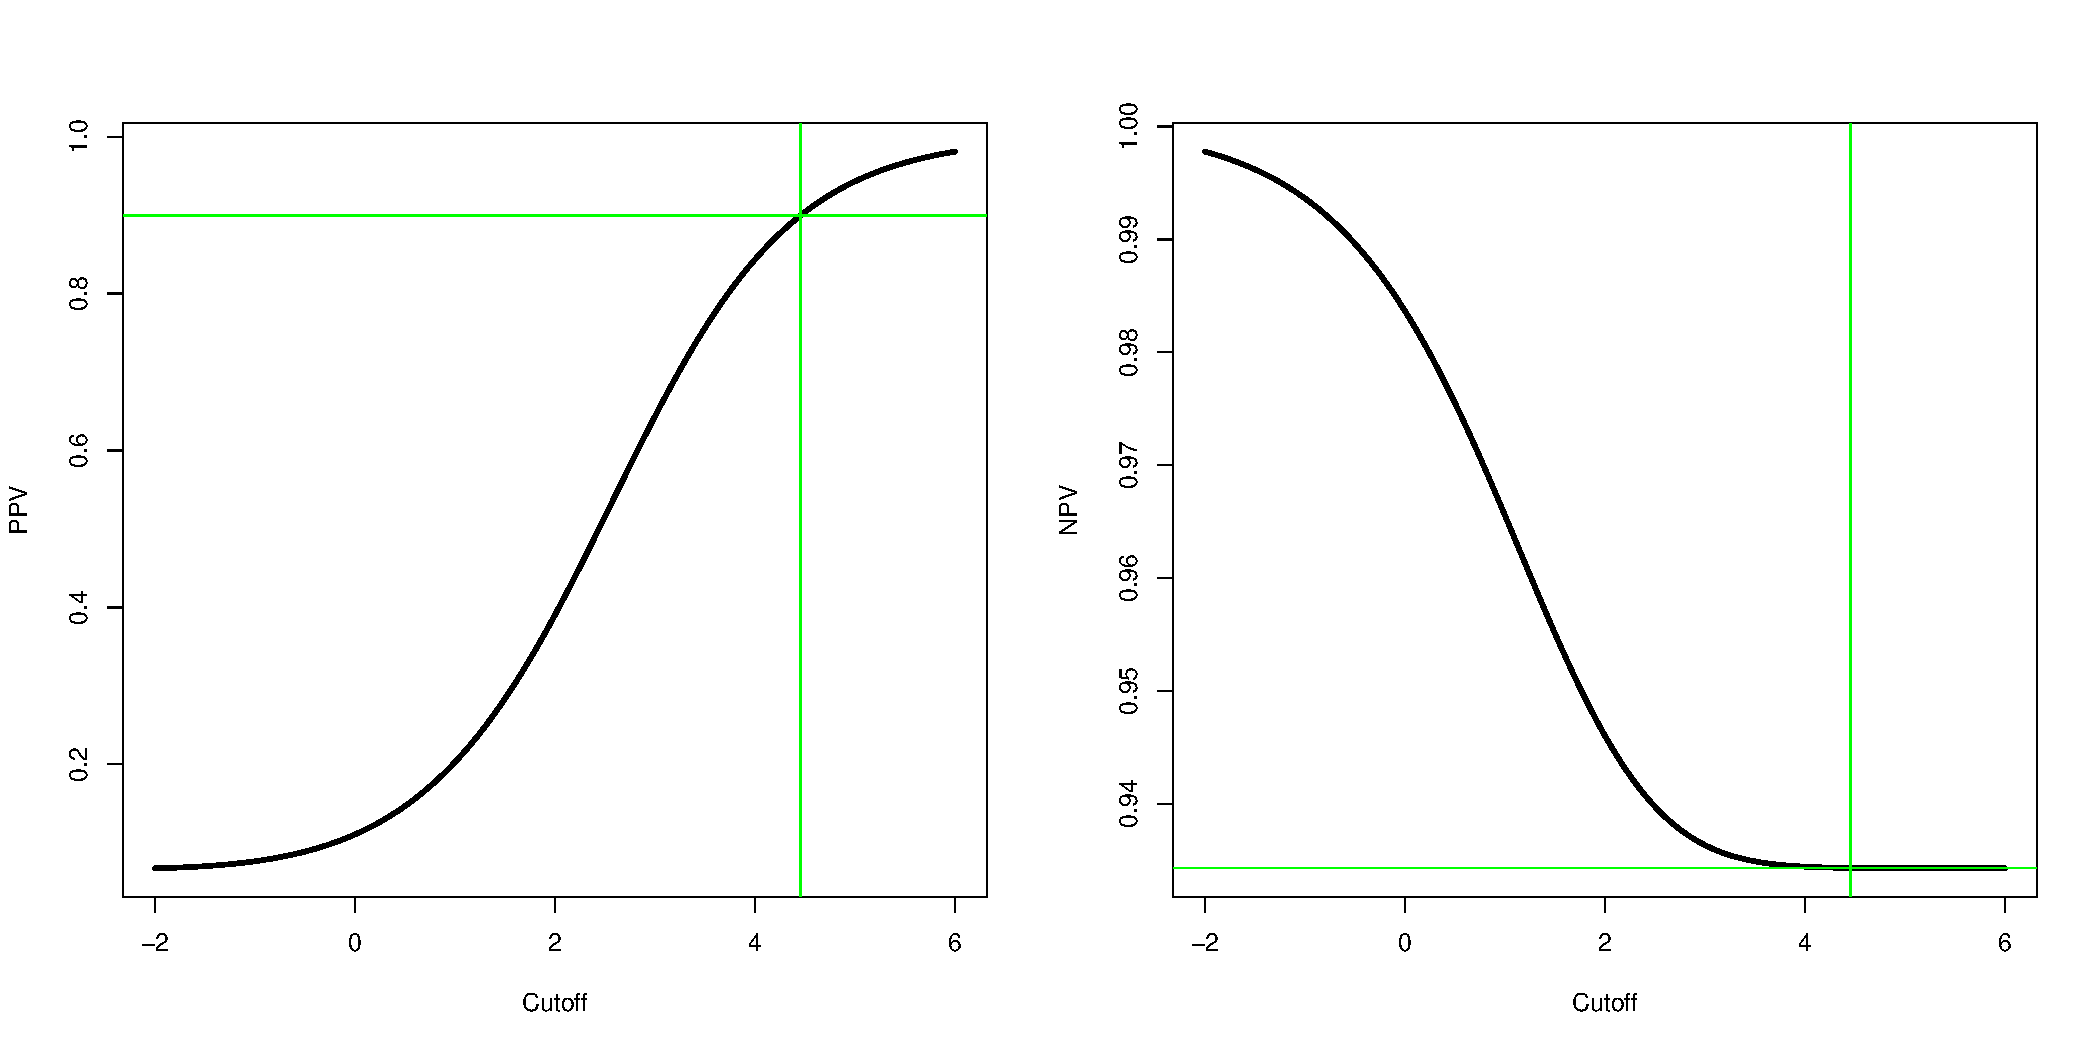
\includegraphics[width=\maxwidth]{figure/unnamed-chunk-12} 

\end{knitrout}

The $Y$ values that satisify this cutoff are
\begin{knitrout}
\definecolor{shadecolor}{rgb}{0.969, 0.969, 0.969}\color{fgcolor}\begin{kframe}
\begin{alltt}
\hlstd{y[y} \hlopt{>} \hlstd{c_star]}
\end{alltt}
\begin{verbatim}
## [1] 4.841
\end{verbatim}
\end{kframe}
\end{knitrout}

Thus there is only one value of the $Y_i$ that should be further investigated. 
\end{proof}
\end{enumerate}
\end{enumerate}
\end{document}
